% Intro
% =====
%
% Contents
% ========
% 
% - Cryptography
%   - Definition
%   - History
%   - Mathematics became the support of cryptography
%   - How finite fields are in the center of that
%
% - Finite fields arithmetic
%   - Representation on a computer
%   - Bases, basic operations
%
% - Lattices of finite fields
%   - The isomorphism problem (results, algos, history)
%   - Effective lattices in CAS: Magma
%   - The algebraic closure (the different results about that, see Luca's HDR
%   probably to have some background)

This introduction is intended to all readers, not only mathematicians. Those
eager to learn more about the technical details or the mathematics behind the
exposed subjects can do so by reading the articles and books for which we give
references. Of course, this thirst for mathematics can also be fulfilled (up to
a point) by reading the next chapters of this thesis.

\minitoc
% TODO
% ====
%
% Find an illustration (something linked with crypto preferably)
\clearpage

During my PhD, I would always explain to non-mathematicians that I was doing a
PhD in \emph{cryptography}. This is in fact an elaborate lie, because even if
the words ``cryptography'' and ``cryptanalysis'' are among those composing
the title of this work: \emph{Efficient arithmetic for cryptography and
cryptanalysis}, the thesis is definitely more oriented towards the two first
words: \emph{efficient arithmetic}. Still, cryptography is the motivation and
sometimes inspiration for this work. The problems we focus on either have their
roots or have applications in cryptography, thus we begin by explaining what it
is.

\section{Cryptography}

As we are social animals, we often need to communicate with each other.
Sometimes, we want our communications to be secret: the reasons behind this
wish are multiple: military informations, business, secret love stories, banking
informations, personnal medical informations, and so on... Cryptography is the
practice and study of the techniques used to secure communications, in the
presence of third parties called \emph{adversaries}. Historically, cryptography
focused on \emph{encryption} of messages (message confidentiality), \ie making
the message unreadable for someone intercepting or eavesdropping it. For the
rightful recipient of the message to be able to read the message, he or she had
to be able to \emph{decrypt} (we also say \emph{decipher}) the message. It was
only possible when both the sender and the receiver of the message shared a
secret beforehand, the secret was then used to both cipher and decipher the
message. In a cryptographic protocol, the common secret is called a
\emph{key}, because the encryption is viewed as some padlock. This encryption
method is called \emph{symmetric cryptography} because both participants share
the same key. The situation is summed up in Figure~\ref{fig:crypto-sym}.
\begin{figure}[h]
  \centering
  \begin{tikzpicture}
    \node (msg) at (0,0) {Message};
    \node (msg-enc) at (6,0) {Encrypted message};
    \node (msg-rec) at (12,0) {Message};
    \node (secret) at (6, 2) {Secret};
    \node (enc) at (2.15,1.8) {Encryption};
    \node (dec) at (9.75,1.8) {Decryption};

    \draw[->] (msg) -- (msg-enc);
    \draw[->] (msg-enc) -- (msg-rec);
    \draw[->] (secret) to[bend right] (2.2,0);
    \draw[->] (secret) to[bend left] (9.8,0);
    \node (a) at (2.2,1) {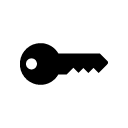
\includegraphics[scale=0.3]{img/key-128.png}};  
    \node (b) at (9.8,1) {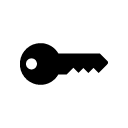
\includegraphics[scale=0.3]{img/key-128.png}};  
    \node (c) at (6,-1) {
\includegraphics[scale=0.05]{img/lock-128.png}};  
  \end{tikzpicture}
  \caption{The general strategy of a symmetric cryptography protocol.}
  \label{fig:crypto-sym}
\end{figure}
One famous example of an old cryptography protocol is the Caesar cipher, in
which each letter of the message is replaced by another letter. All the letters
are shifted by a constant number $n$ of positions down the alphabet. For
example, with $n=3$, the letter D becomes A, the letter E becomes B, the letter
F becomes C, and so on. This encryption protocol is named after Julius Caesar,
who was using it to communicate with his generals with the shift $n=3$. In
Figure~\ref{fig:caesar}, we draw the correspondence between the letters using
the shift $n=3$. The outer ring represent the letters in the \emph{plaintext}
(the original text, without encryption) while the inner ring represent the
letters in the \emph{cyphertext} (the text after the encryption).
\begin{figure}[h]
  \centering
  \begin{tikzpicture}[x=1em,y=1em]
%   set up
    \pgfmathsetmacro\angdiv{360/26}
    \pgfmathtruncatemacro\caeser{3} % Input Caeser shift here! (positive for clockwise)
    \coordinate (n-0) at (90+\angdiv/2:7) {};
    \coordinate (m-0) at (90-\caeser*\angdiv+\angdiv/2:5) {};
%   draw Caeser diagram
    \draw circle [radius=8] circle [radius=6.5] circle [radius=6]  circle [radius=4.5]
        \foreach \i in {0,...,25}{%
            ($({90-(\i-1/2)*\angdiv}:8)$) -- ($(({90-(\i-1/2)*\angdiv}:6.5)$)
            ($({90-(\i-1/2)*\angdiv}:4.5)$) -- ($(({90-(\i-1/2)*\angdiv}:6)$)
        };
    \foreach [count=\a from 0] \text in {A,B,...,Z}{
        \pgfmathtruncatemacro\b{\a+1}%
        \path [curved text=\text] (n-\a) arc [start angle=90-(\a-1/2)*\angdiv, delta angle=-\angdiv, radius=7] node (n-\b) {};
        \path [curved text=\text] (m-\a) arc [start angle=90-(\a+\caeser-1/2)*\angdiv, delta angle=-\angdiv, radius=5] node (m-\b) {}; % Inner circle
    }
%   draw arrow
    \draw [-latex, thick] (65:9.5) to[bend left=20,edge label=$+3$] (40:9.5);
    \end{tikzpicture}
  \caption{Representation of the Caesar cipher with a shift $n=3$.}
  \label{fig:caesar}
\end{figure}
In this example, the secret key of the protocol is the shift parameter $n$: if
you know $n$, you know both how to encrypt a message and how to decrypt one.
Caesar cipher is simple enough to be executed by a machine, but it is not used
nowadays. Indeed, the number of keys one can choose when using Caesar cipher is
rather small, so an adversary (a spy, an ennemy...) can easily guess what it is
after spending enough time trying all the possibilities. One could even ask a
computer to search for all the possible keys, thus recovering it even faster.
That is why, in modern cryptography, the number of possible keys must be way
bigger than this. For example, the standard protocol for symmetric encryption,
called AES (for Advanced Encryption Standard), was designed in 1999~\cite{DR99,
DR02} and can be used with $2^{128}, 2^{192}$ or $2^{256}$ different possible
keys, depending on the version used. The smallest of these number can also be
written as
\[
  2^{128} = 340282366920938463463374607431768211456,
\]
when a billion looks like
\[
  10^{9} = 1000000000,
\]
so they are really big numbers.

The number of possible keys is not the only thing that changed since Julius
Caesar. First, communication is now essentially numerical, thus cryptography is
now a part of computer science. This is very important because it means that the
work in this thesis is also oriented towards computer science: we want to obtain
mathematical results that are effective, \ie usable by a computer.
Second, the scope of cryptography is now larger.
In modern cryptography, symmetric encryption is only one field of
cryptography, and there are many more aspects, such as asymmetric
encryption (also called \emph{public-key} encryption), data integrity,
anthentification, digital signatures (the list is not exhaustive). We will not
explain all these terms, but the interested reader can look at the introductions
on each of these subjects in~\cite{MVOV18}, for example. An important change in
cryptography occured in 1976 with the seminal article \emph{New Directions in
Cryptography}~\cite{DH76} by Diffie and Hellman, with the invention of so called
public key cryptography. We briefly present public key encryption, in order to
compare it to symmetric encryption.

One of the main drawback about symmetric encryption is that the two
protagonists must have a secret in common in order to be able to securely
communicate. They can meet in person and agree on a secret, but this is not
always possible, for example if they live very far away of each other. They
could also find another way of communication, but then they cannot encrypt their
communication, because they do not share a secret yet and they want to
communicate precisely in order to share one. Thus, the problem of sharing a
secret seems to be unsolvable. In fact, public key encryption is an answer to
this problem, because it allows to encrypt messages without the need for a
common secret. The elegant idea of Diffie and Hellman is to break the symmetry
between the participants (we will call them Alice and Bob, since it is
traditional to do so in cryptography). Instead of agreeing on a common key, only
one participant (for example Alice) creates a \emph{pair} of keys: one of them
is public and can be transmitted to anyone, while the other is private and must
be known by Alice only. With the public key, one can encrypt a message, while
the private key is necessary in order to decrypt an encrypted message. Using
such a system, everyone is able to send encrypted messages to Alice, because the
key used to do so is public, but only Alice can decrypt them. Thus, the
communications are secure.
\begin{figure}[h]
  \centering
  \begin{tikzpicture}
    \node (msg) at (0,0) {Message};
    \node (msg-enc) at (6,0) {Encrypted message};
    \node (msg-dec) at (12,0) {Decrypted message};
    \node (bob) at (0,2) {Bob};
    \node (alice) at (12, 2) {Alice};
    \node (key-pub) at (5, 2) {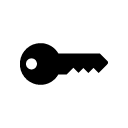
\includegraphics[scale=0.3]{img/key-128.png}};
    \node (key-pub-txt) at (5, 3) {Public key};
    \node (key-pri) at (7, 2) {
\includegraphics[scale=0.065]{img/key-512.png}};
    \node (key-pri-txt) at (7, 3) {Private key};
    \draw[->] (msg) -- (msg-enc);
    \draw[->] (msg-enc) -- (msg-dec);
    \draw[->] (bob) to[bend left, edge label=Encrypts] (2.5,0);
    \node (key-pub2) at (2.2, .8) {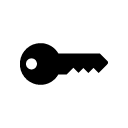
\includegraphics[scale=0.3]{img/key-128.png}};
    \draw[->] (alice) to[bend right, edge label = Decrypts] (9,0);
    \node (key-pri2) at (9.4, .8) {
\includegraphics[scale=0.065]{img/key-512.png}};
    \draw[->] (alice) to (8,2);
    \node (c) at (9.5, 2.3) {Creates};
  \end{tikzpicture}
  \caption{General concept of public-key encryption.}
  \label{fig:crypto-asym}
\end{figure}

\section{Finite fields arithmetic}

\section{Lattices of finite fields}
%
